%% bare_jrnl.tex
%% V1.4a
%% 2014/09/17
%% by Michael Shell
%% see http://www.michaelshell.org/
%% for current contact information.
%%
%% This is a skeleton file demonstrating the use of IEEEtran.cls
%% (requires IEEEtran.cls version 1.8a or later) with an IEEE
%% journal paper.
%%
%% Support sites:
%% http://www.michaelshell.org/tex/ieeetran/
%% http://www.ctan.org/tex-archive/macros/latex/contrib/IEEEtran/
%% and
%% http://www.ieee.org/

%%*************************************************************************
%% Legal Notice:
%% This code is offered as-is without any warranty either expressed or
%% implied; without even the implied warranty of MERCHANTABILITY or
%% FITNESS FOR A PARTICULAR PURPOSE! 
%% User assumes all risk.
%% In no event shall IEEE or any contributor to this code be liable for
%% any damages or losses, including, but not limited to, incidental,
%% consequential, or any other damages, resulting from the use or misuse
%% of any information contained here.
%%
%% All comments are the opinions of their respective authors and are not
%% necessarily endorsed by the IEEE.
%%
%% This work is distributed under the LaTeX Project Public License (LPPL)
%% ( http://www.latex-project.org/ ) version 1.3, and may be freely used,
%% distributed and modified. A copy of the LPPL, version 1.3, is included
%% in the base LaTeX documentation of all distributions of LaTeX released
%% 2003/12/01 or later.
%% Retain all contribution notices and credits.
%% ** Modified files should be clearly indicated as such, including  **
%% ** renaming them and changing author support contact information. **
%%
%% File list of work: IEEEtran.cls, IEEEtran_HOWTO.pdf, bare_adv.tex,
%%                    bare_conf.tex, bare_jrnl.tex, bare_conf_compsoc.tex,
%%                    bare_jrnl_compsoc.tex, bare_jrnl_transmag.tex
%%*************************************************************************


% *** Authors should verify (and, if needed, correct) their LaTeX system  ***
% *** with the testflow diagnostic prior to trusting their LaTeX platform ***
% *** with production work. IEEE's font choices and paper sizes can       ***
% *** trigger bugs that do not appear when using other class files.       ***
% The testflow support page is at:
% http://www.michaelshell.org/tex/testflow/



\documentclass[journal]{IEEEtran}
%
% If IEEEtran.cls has not been installed into the LaTeX system files,
% manually specify the path to it like:
% \documentclass[journal]{../sty/IEEEtran}





% Some very useful LaTeX packages include:
% (uncomment the ones you want to load)


% *** MISC UTILITY PACKAGES ***
%
%\usepackage{ifpdf}
% Heiko Oberdiek's ifpdf.sty is very useful if you need conditional
% compilation based on whether the output is pdf or dvi.
% usage:
% \ifpdf
%   % pdf code
% \else
%   % dvi code
% \fi
% The latest version of ifpdf.sty can be obtained from:
% http://www.ctan.org/tex-archive/macros/latex/contrib/oberdiek/
% Also, note that IEEEtran.cls V1.7 and later provides a builtin
% \ifCLASSINFOpdf conditional that works the same way.
% When switching from latex to pdflatex and vice-versa, the compiler may
% have to be run twice to clear warning/error messages.






% *** CITATION PACKAGES ***
%
%\usepackage{cite}
% cite.sty was written by Donald Arseneau
% V1.6 and later of IEEEtran pre-defines the format of the cite.sty package
% \cite{} output to follow that of IEEE. Loading the cite package will
% result in citation numbers being automatically sorted and properly
% "compressed/ranged". e.g., [1], [9], [2], [7], [5], [6] without using
% cite.sty will become [1], [2], [5]--[7], [9] using cite.sty. cite.sty's
% \cite will automatically add leading space, if needed. Use cite.sty's
% noadjust option (cite.sty V3.8 and later) if you want to turn this off
% such as if a citation ever needs to be enclosed in parenthesis.
% cite.sty is already installed on most LaTeX systems. Be sure and use
% version 5.0 (2009-03-20) and later if using hyperref.sty.
% The latest version can be obtained at:
% http://www.ctan.org/tex-archive/macros/latex/contrib/cite/
% The documentation is contained in the cite.sty file itself.

\usepackage{hyperref}

\usepackage{color}


% *** GRAPHICS RELATED PACKAGES ***
%
\ifCLASSINFOpdf
   \usepackage[pdftex]{graphicx}
  % declare the path(s) where your graphic files are
  % \graphicspath{{../pdf/}{../jpeg/}}
  % and their extensions so you won't have to specify these with
  % every instance of \includegraphics
  % \DeclareGraphicsExtensions{.pdf,.jpeg,.png}
\else
  % or other class option (dvipsone, dvipdf, if not using dvips). graphicx
  % will default to the driver specified in the system graphics.cfg if no
  % driver is specified.
   \usepackage[dvips]{graphicx}
  % declare the path(s) where your graphic files are
  % \graphicspath{{../eps/}}
  % and their extensions so you won't have to specify these with
  % every instance of \includegraphics
  % \DeclareGraphicsExtensions{.eps}
\fi
% graphicx was written by David Carlisle and Sebastian Rahtz. It is
% required if you want graphics, photos, etc. graphicx.sty is already
% installed on most LaTeX systems. The latest version and documentation
% can be obtained at: 
% http://www.ctan.org/tex-archive/macros/latex/required/graphics/
% Another good source of documentation is "Using Imported Graphics in
% LaTeX2e" by Keith Reckdahl which can be found at:
% http://www.ctan.org/tex-archive/info/epslatex/
%
% latex, and pdflatex in dvi mode, support graphics in encapsulated
% postscript (.eps) format. pdflatex in pdf mode supports graphics
% in .pdf, .jpeg, .png and .mps (metapost) formats. Users should ensure
% that all non-photo figures use a vector format (.eps, .pdf, .mps) and
% not a bitmapped formats (.jpeg, .png). IEEE frowns on bitmapped formats
% which can result in "jaggedy"/blurry rendering of lines and letters as
% well as large increases in file sizes.
%
% You can find documentation about the pdfTeX application at:
% http://www.tug.org/applications/pdftex





% *** MATH PACKAGES ***
%
%\usepackage[cmex10]{amsmath}
% A popular package from the American Mathematical Society that provides
% many useful and powerful commands for dealing with mathematics. If using
% it, be sure to load this package with the cmex10 option to ensure that
% only type 1 fonts will utilized at all point sizes. Without this option,
% it is possible that some math symbols, particularly those within
% footnotes, will be rendered in bitmap form which will result in a
% document that can not be IEEE Xplore compliant!
%
% Also, note that the amsmath package sets \interdisplaylinepenalty to 10000
% thus preventing page breaks from occurring within multiline equations. Use:
%\interdisplaylinepenalty=2500
% after loading amsmath to restore such page breaks as IEEEtran.cls normally
% does. amsmath.sty is already installed on most LaTeX systems. The latest
% version and documentation can be obtained at:
% http://www.ctan.org/tex-archive/macros/latex/required/amslatex/math/





% *** SPECIALIZED LIST PACKAGES ***
%
%\usepackage{algorithmic}
% algorithmic.sty was written by Peter Williams and Rogerio Brito.
% This package provides an algorithmic environment fo describing algorithms.
% You can use the algorithmic environment in-text or within a figure
% environment to provide for a floating algorithm. Do NOT use the algorithm
% floating environment provided by algorithm.sty (by the same authors) or
% algorithm2e.sty (by Christophe Fiorio) as IEEE does not use dedicated
% algorithm float types and packages that provide these will not provide
% correct IEEE style captions. The latest version and documentation of
% algorithmic.sty can be obtained at:
% http://www.ctan.org/tex-archive/macros/latex/contrib/algorithms/
% There is also a support site at:
% http://algorithms.berlios.de/index.html
% Also of interest may be the (relatively newer and more customizable)
% algorithmicx.sty package by Szasz Janos:
% http://www.ctan.org/tex-archive/macros/latex/contrib/algorithmicx/




% *** ALIGNMENT PACKAGES ***
%
%\usepackage{array}
% Frank Mittelbach's and David Carlisle's array.sty patches and improves
% the standard LaTeX2e array and tabular environments to provide better
% appearance and additional user controls. As the default LaTeX2e table
% generation code is lacking to the point of almost being broken with
% respect to the quality of the end results, all users are strongly
% advised to use an enhanced (at the very least that provided by array.sty)
% set of table tools. array.sty is already installed on most systems. The
% latest version and documentation can be obtained at:
% http://www.ctan.org/tex-archive/macros/latex/required/tools/


% IEEEtran contains the IEEEeqnarray family of commands that can be used to
% generate multiline equations as well as matrices, tables, etc., of high
% quality.




% *** SUBFIGURE PACKAGES ***
%\ifCLASSOPTIONcompsoc
%  \usepackage[caption=false,font=normalsize,labelfont=sf,textfont=sf]{subfig}
%\else
%  \usepackage[caption=false,font=footnotesize]{subfig}
%\fi
% subfig.sty, written by Steven Douglas Cochran, is the modern replacement
% for subfigure.sty, the latter of which is no longer maintained and is
% incompatible with some LaTeX packages including fixltx2e. However,
% subfig.sty requires and automatically loads Axel Sommerfeldt's caption.sty
% which will override IEEEtran.cls' handling of captions and this will result
% in non-IEEE style figure/table captions. To prevent this problem, be sure
% and invoke subfig.sty's "caption=false" package option (available since
% subfig.sty version 1.3, 2005/06/28) as this is will preserve IEEEtran.cls
% handling of captions.
% Note that the Computer Society format requires a larger sans serif font
% than the serif footnote size font used in traditional IEEE formatting
% and thus the need to invoke different subfig.sty package options depending
% on whether compsoc mode has been enabled.
%
% The latest version and documentation of subfig.sty can be obtained at:
% http://www.ctan.org/tex-archive/macros/latex/contrib/subfig/




% *** FLOAT PACKAGES ***
%
%\usepackage{fixltx2e}
% fixltx2e, the successor to the earlier fix2col.sty, was written by
% Frank Mittelbach and David Carlisle. This package corrects a few problems
% in the LaTeX2e kernel, the most notable of which is that in current
% LaTeX2e releases, the ordering of single and double column floats is not
% guaranteed to be preserved. Thus, an unpatched LaTeX2e can allow a
% single column figure to be placed prior to an earlier double column
% figure. The latest version and documentation can be found at:
% http://www.ctan.org/tex-archive/macros/latex/base/


%\usepackage{stfloats}
% stfloats.sty was written by Sigitas Tolusis. This package gives LaTeX2e
% the ability to do double column floats at the bottom of the page as well
% as the top. (e.g., "\begin{figure*}[!b]" is not normally possible in
% LaTeX2e). It also provides a command:
%\fnbelowfloat
% to enable the placement of footnotes below bottom floats (the standard
% LaTeX2e kernel puts them above bottom floats). This is an invasive package
% which rewrites many portions of the LaTeX2e float routines. It may not work
% with other packages that modify the LaTeX2e float routines. The latest
% version and documentation can be obtained at:
% http://www.ctan.org/tex-archive/macros/latex/contrib/sttools/
% Do not use the stfloats baselinefloat ability as IEEE does not allow
% \baselineskip to stretch. Authors submitting work to the IEEE should note
% that IEEE rarely uses double column equations and that authors should try
% to avoid such use. Do not be tempted to use the cuted.sty or midfloat.sty
% packages (also by Sigitas Tolusis) as IEEE does not format its papers in
% such ways.
% Do not attempt to use stfloats with fixltx2e as they are incompatible.
% Instead, use Morten Hogholm'a dblfloatfix which combines the features
% of both fixltx2e and stfloats:
%
% \usepackage{dblfloatfix}
% The latest version can be found at:
% http://www.ctan.org/tex-archive/macros/latex/contrib/dblfloatfix/




%\ifCLASSOPTIONcaptionsoff
%  \usepackage[nomarkers]{endfloat}
% \let\MYoriglatexcaption\caption
% \renewcommand{\caption}[2][\relax]{\MYoriglatexcaption[#2]{#2}}
%\fi
% endfloat.sty was written by James Darrell McCauley, Jeff Goldberg and 
% Axel Sommerfeldt. This package may be useful when used in conjunction with 
% IEEEtran.cls'  captionsoff option. Some IEEE journals/societies require that
% submissions have lists of figures/tables at the end of the paper and that
% figures/tables without any captions are placed on a page by themselves at
% the end of the document. If needed, the draftcls IEEEtran class option or
% \CLASSINPUTbaselinestretch interface can be used to increase the line
% spacing as well. Be sure and use the nomarkers option of endfloat to
% prevent endfloat from "marking" where the figures would have been placed
% in the text. The two hack lines of code above are a slight modification of
% that suggested by in the endfloat docs (section 8.4.1) to ensure that
% the full captions always appear in the list of figures/tables - even if
% the user used the short optional argument of \caption[]{}.
% IEEE papers do not typically make use of \caption[]'s optional argument,
% so this should not be an issue. A similar trick can be used to disable
% captions of packages such as subfig.sty that lack options to turn off
% the subcaptions:
% For subfig.sty:
% \let\MYorigsubfloat\subfloat
% \renewcommand{\subfloat}[2][\relax]{\MYorigsubfloat[]{#2}}
% However, the above trick will not work if both optional arguments of
% the \subfloat command are used. Furthermore, there needs to be a
% description of each subfigure *somewhere* and endfloat does not add
% subfigure captions to its list of figures. Thus, the best approach is to
% avoid the use of subfigure captions (many IEEE journals avoid them anyway)
% and instead reference/explain all the subfigures within the main caption.
% The latest version of endfloat.sty and its documentation can obtained at:
% http://www.ctan.org/tex-archive/macros/latex/contrib/endfloat/
%
% The IEEEtran \ifCLASSOPTIONcaptionsoff conditional can also be used
% later in the document, say, to conditionally put the References on a 
% page by themselves.




% *** PDF, URL AND HYPERLINK PACKAGES ***
%
%\usepackage{url}
% url.sty was written by Donald Arseneau. It provides better support for
% handling and breaking URLs. url.sty is already installed on most LaTeX
% systems. The latest version and documentation can be obtained at:
% http://www.ctan.org/tex-archive/macros/latex/contrib/url/
% Basically, \url{my_url_here}.




% *** Do not adjust lengths that control margins, column widths, etc. ***
% *** Do not use packages that alter fonts (such as pslatex).         ***
% There should be no need to do such things with IEEEtran.cls V1.6 and later.
% (Unless specifically asked to do so by the journal or conference you plan
% to submit to, of course. )


% correct bad hyphenation here
\hyphenation{op-tical net-works semi-conduc-tor}

\def\SA#1{[{\color{red}SA: \it #1}]}
\def\JS#1{[{\color{magenta}JS: \it #1}]}

\usepackage{hyperref}
\hypersetup{
    colorlinks = true
}
\begin{document}
%
% paper title
% Titles are generally capitalized except for words such as a, an, and, as,
% at, but, by, for, in, nor, of, on, or, the, to and up, which are usually
% not capitalized unless they are the first or last word of the title.
% Linebreaks \\ can be used within to get better formatting as desired.
% Do not put math or special symbols in the title.
\title{Unsupervised Learning for Computational Phenotyping}

% TODO: Another project title?

%
%
% author names and IEEE memberships
% note positions of commas and nonbreaking spaces ( ~ ) LaTeX will not break
% a structure at a ~ so this keeps an author's name from being broken across
% two lines.
% use \thanks{} to gain access to the first footnote area
% a separate \thanks must be used for each paragraph as LaTeX2e's \thanks
% was not built to handle multiple paragraphs
%

\author{Chris Hodapp (\url{chodapp3@gatech.edu})
  % \thanks{\url{chodapp3@gatech.edu}}
}

% The paper headers
\markboth{CSE8803 Big Data Analytics for Healthcare, Fall 2016}%
{Shell \MakeLowercase{\textit{et al.}}: Bare Demo of IEEEtran.cls for Journals}

% Comments:

% Abstract: 0.8/1 It would be better to reduce the amount of sentences
% about the related works but increase those about your own works in
% this paper. Introduction: 0.8/1 You can also compare other
% unsupervised learning methods such as clustering and matrix/tensor
% factorization. Section "Problem Formulation" could be merged into
% Introductino/Background and Method sections. Method: 1/2 What is 'a'
% in time-warping? and write a equation itself not just cite it,
% e.g. euqation 5. Also, describe the algorithm even though it is
% others work if you used it, e.g. "algorithm 2.1 of the
% aforementioned text". As a result, these makes your appoaches very
% unclear. Result-Data: 0.5/1 Please provide more about the data,
% especially after the study cohort is constructed. Patient-wise
% statistics would be needed, how many patients there are, how
% gender/age are distributed, etc. Result-Performance: 0.5/1 It is not
% on the stage where we can discuss about the performance
% Result-Analysis: 0.5/1 yes, we need more results Conclusion: 0.5/1
% You do not need to explain why you did/could not use some
% libraries. Focus on what you did/could. Although there is not enough
% time, you can just take a look this, an example of unsupervised way
% used LSTM
% http://www.jmlr.org/proceedings/papers/v37/srivastava15.pdf
% Reference: 1/1 Organization/Writing: 0.7/1 Overalll structure is
% okay, but you need to clearly describe your approaches. Currently it
% is difficult to figure out it by reading only your paper. Comment:
% As already noted, the most critical issue now is lack of the result
% itself and its analysis. I hope we can see it in the final paper.

% Review 1:

% [Summary]: This paper is about finding hidden patterns in electronic
% health records. The aim of the paper is to use Big data tools to do
% unsupervised learning on the mimic III data.
% [Strength]
% S1: The explanation of the analysis and implementation is great. The
% use of formulas to describe various functions make it clear to the
% reader that the analysis is correct.
% S2: The feature learning part describes in detail each step of the
% feature extraction. This was a great way for the reader to
% understand the steps involved.
% S3: The loading and selecting data is a great way to show the stats
% about the data and point out some of the nuances in the data.
% [Weakness]
% W1: The figure in the experimental evaluation needs explanation. In
% its current state it isn't clear what information can be extracted
% from the figure.
% W2: The figures should be labeled.
% W3: Tensor flow is mentioned without any prior use of the term or
% tool or any reference to it.
% [Intellectual merit] (what is the novelty of the approach?): The use
% of keras, ufldl.
% [Broader impact] (how important is the proposed problem?) The
% proposed problem is extremely important to the field of big
% data. Being able to extract critical information about patient data
% that is otherwise hidden from the physicians could help save many
% lives.
% [Evaluation] (how comprehensive is their evaluation? how good are
% their results?): Some of the results are still being formulated but
% the evaluation is very comprehensive and I'm sure the author will
% have great results.

% Review 2

% Summary:

% This paper presents example of computational phenotyping by using
% unsupervised learning techniques. It follows a similar approach used
% by Lasko et. al., which focused on discovering disease subtypes of
% Leukemia by analyzing time series of uric acid measurements using
% deep learning framework. This paper used the MIMIC III dataset, and
% focused on the time series measurements of blood pH. One of the
% challenges in getting good time series medical data in clinical
% settings is the sparsity and irregularity of measurements. Like
% Lasko et. al., this paper also used Gaussian Processes for smoothing
% the irregularity of measurements.
% Strengths:
% 1. The paper provides robust references and it seems like
% substantial study and research has been done of existing papers and
% relevant technical concepts that are applicable in this area. It
% appears that the author also reached out to one of the other authors
% (Lasko) of the referenced papers to get additional details.
% 2. Substantial space has been given to explaining and developing
% important pre-processing concepts such as Time Warping, and Gaussian
% Process Regression and choice of the covariance function for this
% problem. The paper considered at least a couple of alternate
% covariance functions and chose one from among those.
% 3. The paper also captures some interesting implementation details
% and references, for example related to the implementation of
% auto-encoders. This should form an interesting area to expound on
% further, as it can be turned into a full fledge tutorial. With the
% stated intent of the author to open source the implementation, this
% may not be a far off goal.
% Weaknesses:
% 1. Some more discussion could be added related to the expected
% clinical outcome of this particular study, and how the results will
% be interpreted. For example, Lasko's paper identified two types of
% leukemia upfront, and they were able to show their unsupervised
% clustering implementation was able to successfully differentiate
% between at least those two, in addition to discovering more
% sub-types. A similar target and evaluation criteria is missing in
% this case; it is not clear what baseline disease sub-types does the
% author expect to discover from measuring blood pH levels. Without
% such criteria, it will not be clear how the quality of any
% discovered clusters or phenotypes should be evaluated.
% 2. It would help to include some discussion of how to interpret the
% included results, even if incomplete. For example, the paper
% presents a figure with different waveforms discovered by a layer of
% the auto-encoder, and the author states that either the neural
% network still requires tuning, or that the input data is
% problematic. However, why the author is saying that is not
% clarified. Maybe including some discussion of what the author was
% expecting would help (this may also be tied to the first point above
% about clearly developing an evaluation criteria).
% 3. Being an interesting and technically deep study, it may be useful
% to complete the paper by using simpler implementation so that more
% interpretable results (such as disease clusters) can be
% included. Eventually more complexity can be added moving forward.
% Intellectual merit: This paper studied the field of computational
% phenotyping through unsupervised learning, and presented the
% challenges of implementing such a system. If the implementation is
% open sourced per the author's intention, it could prove to be an
% important contribution to this area.
% Broader impact: Current phenotyping methods using expert knowledge
% and hand-crafted features are time consuming, constrained by the
% amount of data that can be utilized, and by the known categories of
% diseases and conditions. Unsupervised computational phenotyping
% promises to break these barriers and potentially provide useful
% information in the form of patterns and disease sub-categories for
% clinical purposes. A working open source implementation of such a
% tool has the potential to reduce the barriers to entry in this area,
% and propel innovation and hopefully provide better solutions for
% some of the difficult health care problems.
% Evaluation: The author developed the technical concepts very nicely,
% and it appears they were able to implement significant processing
% logic given the amount of time available. They were able to
% visualize the output from an intermediate layer of encoders, which
% in general is an important step in model interpretation in
% unsupervised learning systems, such as deep learning models. As
% stated above, a clear goal and evaluation criteria in terms of the
% clinical concept targeted in the paper (i.e. blood pH levels) needs
% to be developed in order to interpret and evaluate the results in a
% meaningful way.

% Review 3

% This paper intends to implement and improve upon the work by Lasko
% et al. on computational phenotyping using autoencoding techniques
% with the help of big data tools. This technique hels capture new
% features in timeseries information which might help to provide a
% strong phenotype classifier.
% S1: Extensive description of the techniques developed along with
% appropriate mathematics help back th
% S2: care has been taken to preprocess data that is potentially very
% noisy, before being used for unsupervised learning
% S3: care is taken that hyperparameter tuning is done while
% pre-processing is done, in order to optimize search space and
% generate appropriate generator variables values.

\maketitle

% As a general rule, do not put math, special symbols or citations
% in the abstract or keywords.
\begin{abstract}
With large volumes of health care data comes the research area of
computational phenotyping, making use of techniques such as machine
learning to describe illnesses and other clinical concepts from the
data itself.  The ``traditional'' approach of using supervised
learning relies on a domain expert, and has two main limitations:
requiring skilled humans to supply correct labels limits its
scalability and accuracy, and relying on existing clinical
descriptions limits the sorts of patterns that can be found. For
instance, it may fail to acknowledge that a disease treated as a
single condition may really have several subtypes with different
phenotypes, as seems to be the case with asthma and heart
disease. Some recent papers cite successes instead using unsupervised
learning.  This shows great potential for finding patterns in
Electronic Health Records that would otherwise be hidden and that can
lead to greater understanding of conditions and treatments. This work
implements a method derived strongly from Lasko \emph{et al.}, but
implements it in Apache Spark and Python and generalizes it to
laboratory time-series data in MIMIC-III.  It is released as an
open-source tool for exploration, analysis, and visualization.
\end{abstract}
% TODO: Turn 'will be' to 'is' and actually release it.

% Note that keywords are not normally used for peerreview papers.
\begin{IEEEkeywords}
Big data, Health analytics, Data mining, Machine learning,
Unsupervised learning, Computational phenotyping
\end{IEEEkeywords}
% For peer review papers, you can put extra information on the cover
% page as needed:
% \ifCLASSOPTIONpeerreview
% \begin{center} \bfseries EDICS Category: 3-BBND \end{center}
% \fi
%
% For peerreview papers, this IEEEtran command inserts a page break and
% creates the second title. It will be ignored for other modes.
% \IEEEpeerreviewmaketitle

\section{Introduction \& Background}

The field of \emph{computational phenotyping}\cite{Che2015} has
emerged recently as a way of learning more from the increasing volumes
of Electronic Health Records available, and the volume of this data
ties it in naturally with fields like machine learning and data
mining.  The ``traditional'' approach of supervised learning over
classifications has two noted 

\begin{itemize}
\item{It requires the time and attention of that domain expert in
  order to provide classification information over which to train a
  model, and this requirement on human attention limits the amount of
  data available (and, to an extent, its accuracy.)}
\item{It tends to limit the patterns that can be found to what
  existing classifications acknowledge.  If a disease treated as a
  single condition really has multiple subtypes with different
  phenotypes, the model will not reflect this - for instance, asthma
  and heart disease\cite{Lasko2013}.}
\end{itemize}

Some recent papers\cite{Marlin,Lasko2013,Johnson2016} cite
successes with approaches instead using unsupervised learning on
time-series data.  In Lasko \emph{et al.}\cite{Lasko2013}, such an
approach applied to serum uric acid measurements was able to
distinguish gout and acute leukemia with no prior classifications
given in training.  Marlin \emph{et al.}\cite{Marlin} examines 13
physiological measures from a pediatric ICU (such as pulse oximetric
saturation, heart rate, and respiratory rate). Che \emph{et
  al.}\cite{Che2015} likewise uses ICU data, but focuses on certain
ICD-9 codes rather than mortality.

This approach still has technical barriers.  Time-series in healthcare
data frequently are noisy, spare, heterogeneous, or irregularly
sampled, and commonly Gaussian processes are employed here in order to
condition the data into a more regular form as a pre-processing step.
In \cite{Lasko2013}, Gaussian process regression produces a model
which generates a continuous, interpolated time-series providing both
predicted mean and variance.  In \cite{Ghassemi2015} it is used to
instead derive a latent representation from correlated time-series.
Che \emph{et al.}\cite{Che2015} does not use Gaussian process
regression, but rather fills irregularities in the data by propagating
forward or backward.

Che \emph{et al.}\cite{Che2015} notes that ``shallow'' clustering
models such as Gaussian mixture models (as in \cite{Marlin}) are used
too, deep learning succeeds more here at finding latent factors and
extracting concepts - which is particularly important given the
complexity of bodies and processes.  Lasko \emph{et
  al.}\cite{Lasko2013} applies a two-layer stacked sparse autoencoder
(compared with a five-layer stacked denoising autoencoder in
\cite{Che2015}), but the approach that looks like it could extend to a
deep learner with the addition of layers.

The goal undertaken here was to reimplement a combination of some
earlier results (focusing mainly on that of Lasko \emph{et
  al.}\cite{Lasko2013}) using \href{http://spark.apache.org/}{Apache
  Spark} and the MIMIC-III critical care database\cite{Johnson2016a},
and able to run primarily on a ``standard'' Spark setup such as
\href{https://aws.amazon.com/emr/}{Amazon Elastic MapReduce}.
However, presently it relies on Python in order to use Keras and
scikit-learn for feature learning and t-SNE.

The software behind this work is also released as an open source tool
for accomodating exploration, analysis, and visualization using the
techniques described herein.  % TODO: GitHub link

% Most of the needed algorithms are available in existing machine
% learning libraries in languages such as MATLAB or R, however, these
% are less accessible to the aforementioned ``standard'' setup or may
% be more cumbersome to integrate with Apache Spark.  While Apache
% Spark runs on top of Java/JVM infrastructure and has access to a
% considerable ecosystem of Java-based, relevant libraries do not
% always exist or do not exist in a form which works well with Spark.

% TODO: Mention integration with other languages via SparkR, PySpark,
% Java APIs?

\section{Approach \& Implementation}

The main problems that the implementation tries to address within
these parameters are:

\begin{itemize}
\item{Loading the MIMIC-III database into a form usable from Spark}
\item{Identifying relevant laboratory tests, admissions, and ICD-9
  codes on which to focus}
  % Perhaps de-emphasize this
\item{Preprocessing the time-series data with Gaussian process
  regression}
\item{Using a two-layer stacked sparse autoencoder to perform feature
  learning}
\item{Visualizing the new feature space and identifying potential
  clusters}
\end{itemize}

\subsection{Loading \& Selecting Data}

% TODO: Mention exploratory mode of tool?  Is it needed?

The MIMIC-III database is supplied as a collection of \texttt{.csv.gz}
files (that is, comma-separated values, compressed with gzip).  By way
of \texttt{spack-csv}, Apache Spark 2.x is able to load these files
natively as tabular data, i.e. a \texttt{DataFrame}.  All work
described here used the following tables\cite{Johnson2016a}:

\begin{itemize}
\item \texttt{LABEVENTS}: Timestamped laboratory measurements for patients
\item \texttt{DIAGNOSES\_ICD}: ICD-9 diagnoses for patients (per-admission)
\item \texttt{D\_ICD\_DIAGNOSES}: Information on each ICD-9 diagnosis
\item \texttt{D\_LABEVENTS}: Information on each type of laboratory event
\end{itemize}

% TODO: Cite LOINC?

The process requires two ICD-9 categories, and one LOINC code for a
lab test.  Admissions are filtered to those which contain a lab
time-series of the given LOINC code and containing at least 3 samples,
and to those containing at least one diagnosis of the first ICD-9
category, but none of the second - or, at least one of the second
ICD-9 category, and none of the first.

All processing at this stage was done via Spark's DataFrame
operations, aside from the final conversion to an RDD containing
individual time-series.

\subsection{Preprocessing}

\subsubsection{Time Warping}

The covariance function that is used in Gaussian process regression
(and explained after this section) contains a time-scale parameter
$\tau$ which embeds assumptions on how closely correlated nearby
samples are in time.  This value is assumed not to change within the
time-series - that is, it is assumed to be
\textit{stationary}\cite{Lasko2013}.  This assumption is often
incorrect, but under the assumption that more rapidly-varying things
(that is, shorter time-scale) are measured more frequently, an
approximation can be applied to try to make the time-series more
stationary - in the form of changing the distance in time between
every pair of adjacent samples in order to shorten longer distances,
but lengthen shorter ones\cite{Lasko2013}.  For original distance $d$,
the warped distance is $d'=d^{1/a}+b$, using $a=3, b=0$ (these
values were taken directly from equation 5 of \cite{Lasko2013} and not
tuned further).

Thomas Lasko also related in an email that this assumption (that
measurement frequency was proportional to how volatile the thing being
measured is) is not true for all medical tests.  He referred to
another paper of his\cite{Lasko2015} for a more robust approach,
however, this is not used here.

\subsubsection{Gaussian Process Regression}

In order to condition the irregular and sparse time-series data from
the prior step, Gaussian process regression was used.  The method used
here is what Lasko \emph{et al.}\cite{Lasko2013} described, which in
more depth is the method described in algorithm 2.1 of Rasmussen \&
Williams\cite{Rasmussen2004}.

In brief, Gaussian process regression (GPR) is a Bayesian
non-parametric, or less parametric, method of supervised learning over
noisy observations\cite{Ebden2015,Lasko2013,Rasmussen2004}.  It is not
completely free-form, but it infers a function constrained only by the
mean function (which here is assumed to be 0 and can be ignored) and
the covariance function $k(t,t')$ of an underlying
infinite-dimensional Gaussian distribution.  It is not exclusive to
time-series data, but $t$ is used here as in this work GPR is done
only on time-series data.

That covariance function $k$ defines how dependent observations are on
each other, and so a common choice is the squared
exponential\cite{Ebden2015}:

$$k(t,t') = \sigma_n^2\exp\bigg[\frac{-(t-t')^2}{2l^2}\bigg]$$

Note that $k$ approaches a maximum of $\sigma_n^2$ as $t$ and $t'$ are
further, and $k$ approaches a minimum of 0 as $t$ and $t'$ are closer.
Intuitively, this makes sense for many ``natural'' functions: we
expect closer $t$ values to have more strongly correlated function
values, and $l$ defines the time scale of that correlation.

The rational quadratic function is used here instead as it better
models things that may occur on many time scales\cite{Lasko2013}:

$$k(t,t') = \sigma_n^2\bigg[1+\frac{(t-t')^2}{2\alpha\tau^2}\bigg]^{-\alpha}$$

Rasmussen \& Williams\cite{Rasmussen2004} supplies a formula for
computing the log marginal likelihood of the target values
$\mathbf{y}$ given the inputs $X$ (both $n\times1$ row vectors of
target values and input values, respectively), where $K$ is a $n\times
n$ matrix for which $K_{ij}=k(X_i,X_j)$:

$$\log p(\mathbf{y}|X) = -\frac{1}{2}\mathbf{y}^\top(K+\sigma_n^2I)^{-1}-\frac{1}{2}\log |K+\sigma_n^2I|-\frac{n}{2}\log2\pi$$

An equivalent version that uses Cholesky decomposition rather than
$n\times n$ matrix inversion is given in algorithm 2.1 of the
aforementioned text, and this is what is actually used in the code.

In specific, in order to optimize the hyperparameters $\sigma_n$,
$\tau$, and $\alpha$ of the covariance function, $\sum\log
p(\mathbf{y}|X)$ was roughly maximized over every time-series in the
training set (following the time warping of the prior section) using a
grid search.  The values found for this were $\sigma_n=1.4$,
$\alpha=0.1$, and $\tau=3.55$.

Hyperparameter optimization was likely the most time-consuming step of
processing.  However, this step also is a highly parallelizable one,
and so it was amenable to the distributed nature of Apache Spark.

The values (i.e. $y$) in each individual time-series were standardized
to a mean of 0 and standard deviation of 1, and this standardization
was then reversed on the interpolated values.

% TODO: Put algorithm 2.1 here perhaps rather than just citing it.

\subsubsection{Interpolation}

The remainder of algorithm 2.1 is not reproduced here, but the code
directly implemented this method using the rational quadratic function
(and hyperparameters given above) as the covariance function.  This
inferred for each individual time-series a continuous function
producing predictive mean and variance for any input $t$ (for which
they use the notation $\mathbf{x^*}$ for ``test input'').

As in \cite{Lasko2013}, all of these inferred functions were then
evaluated at a regular sampling of time values (i.e. via the test
input $\mathbf{x^*}$) with padding added before and after each time
series.  The sampling frequency and the amount of padding depends on
the dataset, and so can be specified when running the tool.

In effect, this mapped each individual time-series first to a
continuous function, and then to a new ``interpolated'' time-series
containing predicted mean and variance at the sampled times described
above (a total of 341,819 interpolated time-series samples).  These
interpolated time-series were then the input to later steps.

\subsection{Feature Learning with Autoencoder}

A stacked sparse 2-layer autoencoder was then used to perform feature
learning.  The implementation used here was a combination of what was
described in \cite{Lasko2013} (which closely follows the UFLDL
Tutorial from Stanford\cite{Ng}), and Fran\c cois Chollet's
guide\cite{Chollet} on using the Python library
\href{https://keras.io/}{Keras} to implement autoencoders.
Specifically, Keras was used with
\href{http://deeplearning.net/software/theano/}{Theano} (GPU-enabled)
as the backend.

These autoencoders have a fixed-size input and output, and in order to
accomodate this, fixed-size contiguous patches were sampled from the
interpolated time-series.  As in \cite{Lasko2013}, the patch size was
set to the total number of padded samples, and patches were sampled
uniformly randomly from all contiguous patches.  A total of 18,801
patches were produced here, all of which were then standardized to
mean 0 and variance 1.  70\% of these patches were then selected for
autoencoder training, and the remaining 30\% for validation.

To accomodate this patch size, the autoencoder's input and output
layers had 60 units (as each sample contained both variance and mean).

As in \cite{Lasko2013}, the encoder and decoder layers used sigmoid
encoders and linear decoders, and all hidden layers had 100 units.
Manual experimentation led to L1 activity regularization
(i.e. sparsity constraint) of $5\times10^{-5}$ and L2 weight
regularization of $2\times10^{-4}$.

\begin{figure}
  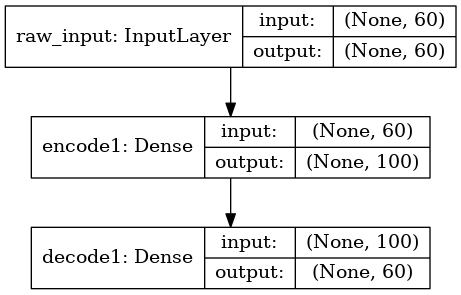
\includegraphics[width=0.7\linewidth]{keras_autoencoder1.eps}
  \caption{First stage of Keras autoencoder}
  \label{fig:keras_autoencoder1}
\end{figure}

\begin{figure}
  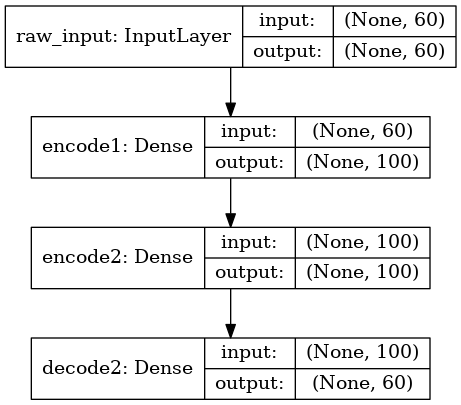
\includegraphics[width=0.7\linewidth]{keras_autoencoder2.eps}
  \caption{Keras network used for autoencoder}
  \label{fig:keras_autoencoder2}
\end{figure}

This network was built up in stages in order to greedy layerwise
train\cite{Ng}.  The first stage was the neural network in figure
\ref{fig:keras_autoencoder1}; this was trained with the raw input data
(at both the input and the output), thus learning ``primary'' hidden
features at the layer \texttt{encode1}.  The first decoder layer
\texttt{decode1} was then discarded and the model extended with
another encoder and decoder, as in figure
\ref{fig:keras_autoencoder2}.

This model then was similarly trained on raw input data, but while
keeping the weights in layer \texttt{encode1} constant.  That is, only
layers \texttt{encode1} and \texttt{decode2} were trained, and in
effect they were trained on ``primary'' hidden features
(i.e. \texttt{encode1}'s activations on raw input).  Following this
was ``fine-tuning''\cite{Ng} which optimized all layers, i.e. the
stacked autoencoder as a whole, again using the raw input data.

The final model then discarded layer \texttt{decode2}, and used the
activations of layer \texttt{encode2} as the learned sparse features.

% TODO: How many iterations?  What algorithms?  What settings?

% From these laboratory measurements and that methodology, I aim to
% produce a transformation to a reduced feature space using a
% combination of Gaussian process regression to condition
% irregularly-sampled input data and autoencoders to learn a
% reduced-dimension form of them.  Using labels such as certain ICD-9
% codes, I will train classifiers from the reduced form, and compute
% their AUCs for these codes.  I will also examine them for apparent
% clusterings that may suggest multiple different phenotypes for some
% label, as seen in \cite[figure 5]{Lasko2013}.

% TODO: t-SNE, sklearn

\section{Experimental Evaluation}

As a test of the tool described in this paper, experiments were run on
a selection of the data.  Particularly, the LOINC code
\texttt{11558-4} (which corresponds to \texttt{ITEMID} of 50820, blood
pH) was used, and the ICD-9 categories 518 (other lung diseases) and
584 (acute renal failure).

This produced a total of 9,035 unique admissions, 8,219 unique
patients, and 187,374 time-stamped samples.  70\% of these admissions
were randomly selected for the training set, and the remaining 30\%
for the testing set.

% TODO: Note padding amount & sampling frequency

% TODO: Note gender, age, percent died?  How many of each ICD-9
% category?

An interesting detail which figure 2 of \cite{Lasko2013} shows is that
the effects of the first layer (\texttt{encode1} here) can be
visualized directly in the form of its weights.  As they form a 60x100
array, each 60-element vector corresponds to a sort of time-series
signature which that unit is detecting.  Figure
\ref{fig:keras_hidden1} shows one such result from training the
network on the subset of the data described here.

\begin{figure}
  \includegraphics[width=\linewidth]{cohort_518_584_11558-4_keras_layer1.eps}
  \caption{Autoencoder first-layer weights, shown as 100 time-series}
  \label{fig:keras_hidden1}
\end{figure}

This shows similar structure as in \cite{Lasko2013} (including
considerable redundancy), but with different sorts of signatures.
Particularly, it seems to single out edges and certain kinds of ramps.

Presently, not many other results are available as further work is
needed.  The resultant features from the autoencoder still need to be
examined alongside their labels, and some further clustering and
visualization done on this.

\section{Conclusions \& Further Work}

This work is still in need of further experimentation and refining in
order to produce meaningful results.  While the tool is meant to work
generally over various subsets of data in MIMIC-III (and similar
datasets with some modification), it may still require considerable
tuning.

Several optimizations also may help.  For instance, hyperparameter
optimization is currently done with a grid search, but would more
sensibly done with a more intelligent optimization algorithm (such as
SGD).  The time warping function has parameters that could be tuned,
or more extensive changes\cite{Lasko2015} could be made to try to make
the time-series more stationary.  Other covariance functions may be
more appropriate as well.

The original intention of running as much as possible within Apache
Spark on ``standard'' infrastructure such as
\href{https://aws.amazon.com/emr/}{Amazon EMR} or
\href{https://databricks.com/}{Databricks} was not fully met.  Further
integration with Apache Spark still is possible; the autoencoders
perhaps could be implemented in
\href{https://deeplearning4j.org/}{DL4J} (a native Java library
supporting Apache Spark) or Spark's built-in \texttt{pyspark} support
may allow closer integration with Keras and scikit-learn.

Some other areas should perhaps be explored further too.  One
incremental change is in the use of multiple-task Gaussian processes
(MTGPs); the work done here handles only individual time-series, while
MIMIC-III is rich in parallel time-series that correlate with each
other.  Ghassemi \emph{et al.}\cite{Ghassemi2015} explored the use of
MTGPs to find a latent representation of multiple correlated
time-series, but did not use this representation for subsequent
feature learning.  Another incremental change is in the use of
Variational Autoencoders (VAEs) to learn a feature space that is
sufficiently low-dimensional that techniques such as t-SNE are not
required for effective visualization.

A more extensive change could involve using recurrent neural networks
(RNNs).  Deep networks such as RNNs such as Long Short-Term Memories
(LSTMs) have shown promise in their ability to more directly handle
sequences\cite{Sutskever2014} and clinical time-series data, including
handling missing data\cite{Lipton2015, Lipton2015a, Lipton2016}.
However, they are primarily used for supervised learning, but could
potentially be treated similarly as autoencoders (as in
\cite{Klapper-Rybicka2001}), that is, trained with the same input and
output data in order to learn a reduced representation of the input.
This approach would avoid some of the need to perform Gaussian Process
Regression, however, it still may not cope well with time-series data
that is very irregular.

\section*{Acknowledgment}
Thank you to Dr. Jimeng Sun and the TAs for their time and effort in
this course.

% TODO Fix the URLs so that they display in the bibliography!

\bibliography{cse8803_report,cse8803_report_websites}
\bibliographystyle{abbrv}

\end{document}
